\section{Ordinary Differential Equations}

Let $x$ be the position of a particle in one dimension, and let $t$ be time.

An Ordinary Differential Equation specifies a velocity $v(t, x)$ at each point
in $(t, x)$ space. Thus an ODE contains all the information needed to animate
the motion of the particle, starting from any point $(t_0, x_0)$.

The solution to an ODE is a function $x = \varphi(t)$ that describes a motion
of the particle having the specified velocities at each point it passes
through. I.e., if $x = \varphi(t)$ is a solution, then
\begin{align*}
  \frac{\d \varphi}{\dt} = v(t, \varphi(t)) ~~~~~~~~~~~~~\text{for all $t$}.
\end{align*}

The phase space of this problem is the set of all possible $(x, v)$ values.?

\subsection{Special cases}
\subsubsection{Velocity depends on time only}
\begin{align*}
  \dxdt = v(t)
\end{align*}
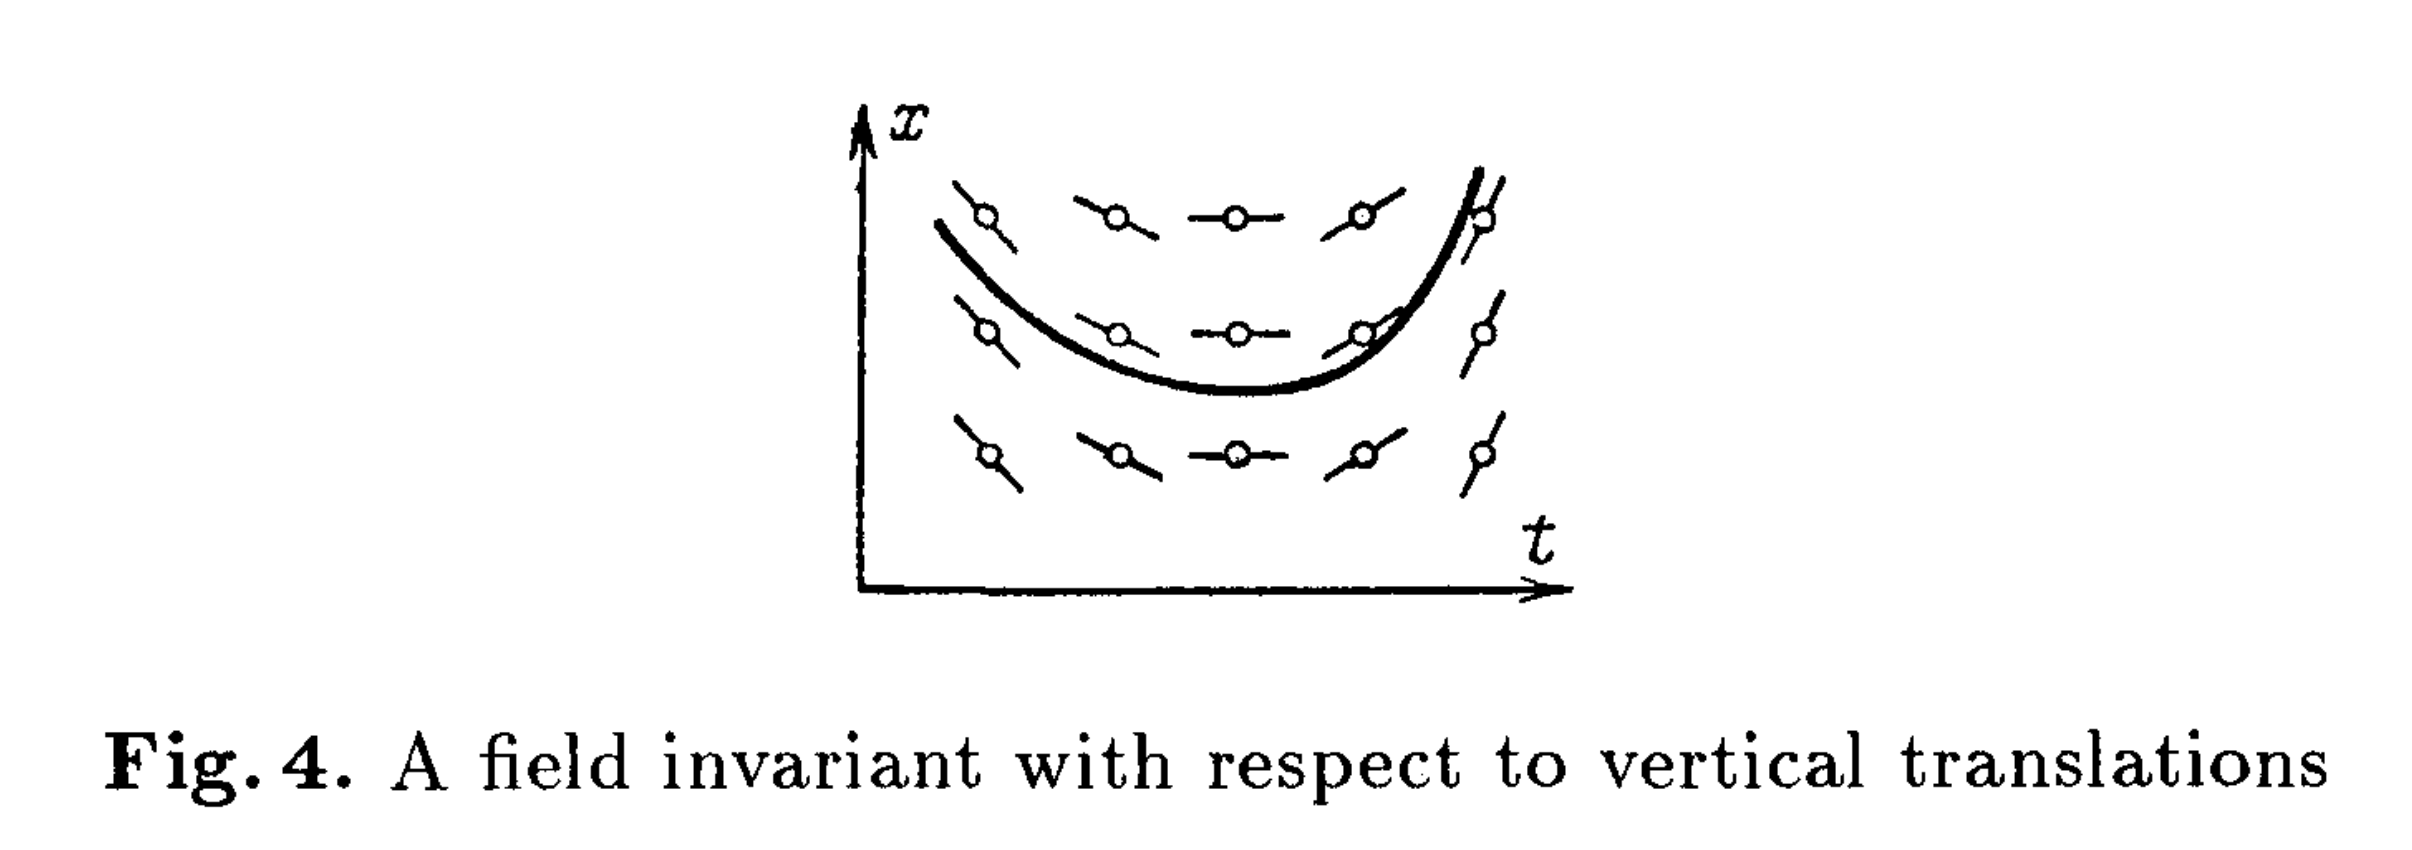
\includegraphics[width=340pt]{img/differential-equations-1-direction-field.png}\\
To find functions that solves this, we find the antiderivative:
\begin{align*}
  \int \dxdt \dt := x(t) + C = \int v(t) \dt
\end{align*}

\subsubsection{Velocity depends on location only (autonomous)}
\begin{align*}
  \dxdt = v(x)
\end{align*}
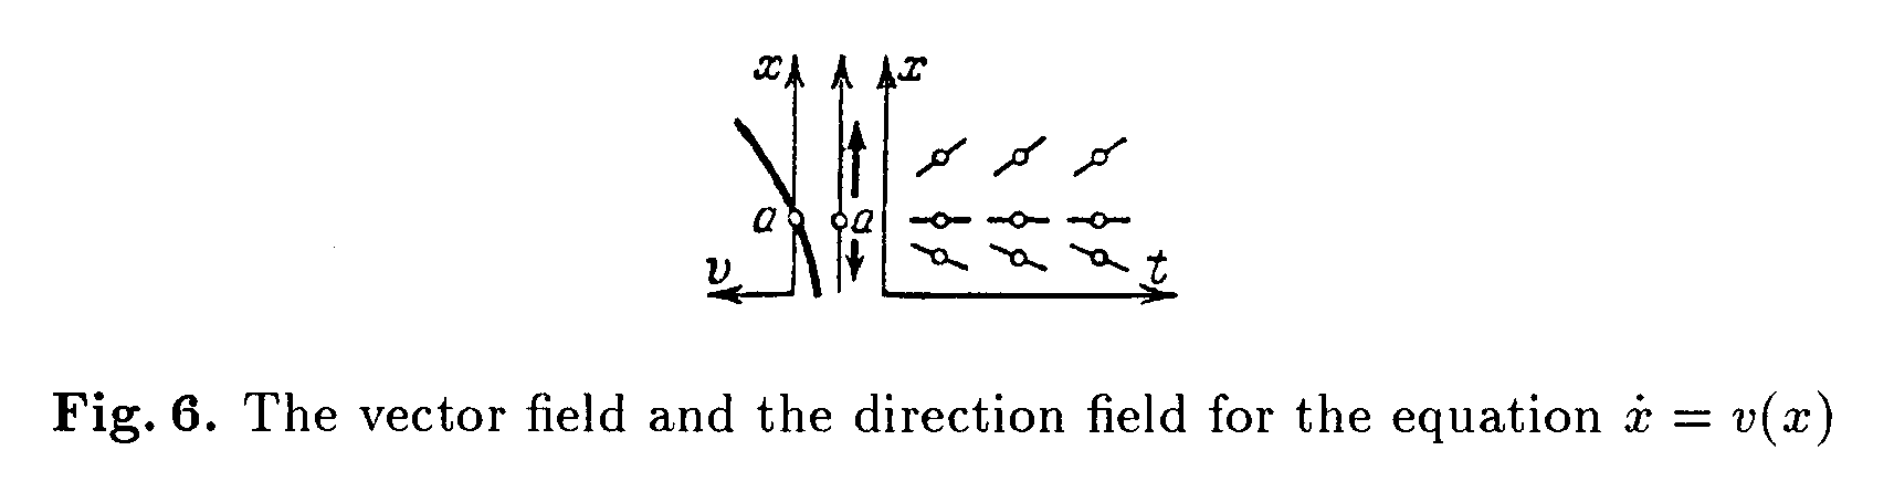
\includegraphics[width=400pt]{img/differential-equations-2-direction-field.png}\\


\section{Examples}
\subsection{C$^{14}$ dating}
\begin{mdframed}
  In a living organism the amount of C$^{14}$, as a proportion of all the
  C$^{12}$ and C$^{14}$, is expected to be a known constant $p_0$. After death,
  C$^{14}$ decays to C$^{12}$. How old is a specimen with proportion $p_1$ of
  C$^{14}$?
\end{mdframed}
Let $\lambda$ be the rate at which one atom of C$^{14}$ decays in atoms/sec. So
in a sample of $N$ atoms, the expected number to decay in one second is
$N\lambda$.

Let $N(t)$ be the number of C$^{14}$ atoms remaining at time $t$. We can
specify the model as a first-order ODE:
\begin{align*}
\frac{\d N}{\dt} = -N\lambda.
\end{align*}
Equivalently, dividing by the constant total number of carbon atoms,
\begin{align*}
\frac{\d p}{\dt} = -p\lambda,
\end{align*}
where $p(t)$ is the proportion of C$^{14}$ at time $t$.

It's easy to find a family of functions $p(t)$ that satisfies this differential equation. Since
\begin{align*}
  \frac{1}{p(t)} \frac{\d p}{\dt} = -\lambda,
\end{align*}
it must be the case that their antiderivatives are the same, up to a constant:
\begin{align*}
  \log(p(t)) &= -\lambda t + C\\
  p(t)  &= Ae^{-\lambda t}.
\end{align*}
Further, the expected proportion in a living organism determines a particular
function as the solution:
\begin{align*}
  p(0) = p_0 = Ae^{-\lambda . 0}
\end{align*}
so $A = p_0$ and the solution is
\begin{align*}
  p(t)  &= p_0e^{-\lambda t}.
\end{align*}
So the estimated age of a sample with proportion $p_1$ is
\begin{align*}
  t = \frac{1}{\lambda}\log\(\frac{p_0}{p_1}\).
\end{align*}


\begin{align*}

\end{align*}

\section{Arnold - Problems}
\subsection{}
\begin{mdframed}
  At what altitude is the density of the air one half of that at the surface of
  the Earth? Regard temperature as constant. One cubic meter of air at the
  Earth's surface weighs 1250g.
\end{mdframed}
\begin{align*}
  \rho(0) = 1250\\
  &=
\end{align*}